\chapter{Planificación}
\label{chap:planificacion}

\lettrine{E}{}n este capítulo se presentan las metodologías de desarrollo elegidas para la realización del proyecto, así como los costes y la organización temporal.

\section{Metodología de desarrollo}

Se seleccionó \textbf{Scrum} \cite{sachdeva2016scrum} como la metodología para este proyecto. Es un enfoque ágil para el desarrollo de software que tiene como objetivo administrar proyectos con flexibilidad y enfocándose en maximizar el retorno de la inversión (ROI). Scrum fue creado alrededor de 1986 por \textbf{Ikujiro Nonaka e Hirotaka Takeuchi}, inspirado en una investigación hecha en varias compañías que estaban implementando un enfoque laboral innovador. Este marco de referencia establece un grupo de eventos, prácticas y roles, y puede ser utilizado como punto de inicio para definir el procedimiento de producción que un equipo de trabajo empleará en un proyecto.


Los principios de Scrum se centran en:

\begin{itemize}
\item \textbf{Control empírico de procesos:} Se basa en la transparencia, inspección y adaptación para aprender a través de la experimentación, especialmente en situaciones donde el problema no está claro.
\item \textbf{Autoorganización:}  Los equipos logran un mayor valor cuando se autoorganizan, lo que fomenta una mejor participación, responsabilidad compartida y un entorno creativo propicio para el crecimiento. 
\item \textbf{Colaboración:} Destaca la importancia de la conciencia, articulación y apropiación en el trabajo colaborativo, involucrando a equipos, clientes y partes interesadas para crear valor compartido.
\item \textbf{ Priorización basada en valores:} Se enfoca en ofrecer el máximo valor comercial desde el principio hasta el final del proyecto.
\item \textbf{Timeboxing:} El tiempo se considera una restricción importante en Scrum y se utiliza para gestionar eficazmente la planificación y ejecución del proyecto.
\item \textbf{Desarrollo iterativo:} Se centra en gestionar cambios y crear productos que satisfagan las necesidades del cliente, delineando las responsabilidades del propietario del producto y la organización en el desarrollo iterativo.
\end{itemize}

\begin{figure}[hp!]
  \centering
  \includegraphics[width=0.75\textwidth]{imaxes/3_SCRUM.png}
  \caption[Marco de trabajo SCRUM]{Marco de trabajo SCRUM. \textit{Fuente: \cite{AusumScrum2024}}}
  \label{fig:3_SCRUM}
\end{figure}


\section{Planificación del proyecto}

Para planificar el desarrollo del proyecto, se utilizó un \textbf{diagrama de Gantt} \cite{diagramaGantt}. Este gráfico ofrece un cronograma del proyecto donde se pueden visualizar las fechas de inicio y finalización de las tareas y hitos. Cada tarea se representa con una barra horizontal que indica su duración, con fechas de inicio y finalización acordadas antes del inicio del proyecto.

En la siguiente figura \ref{fig:3_DiagramaGantt}, se muestra el inicio y la finalización del proyecto. La finalización está programada una semana antes de la entrega para permitir una revisión exhaustiva.

Es importante destacar que se llevan a cabo reuniones semanales con el tutor para realizar un seguimiento del progreso del proyecto.

Se ha implementado la metodología Scrum en el desarrollo del proyecto. Durante la organización de este proyecto se seguirán las siguientes etapas distintivas:
\begin{itemize}
\item \textbf{Sprint Planning:} En este comienzo de Scrum se trata de detallar las responsabilidades de los integrantes del equipo y estimar el tiempo para completarlas.
\item \textbf{Scrum Team Meeting:}  Reuniones informativas y diarias realizadas por los equipos laborales para revisar avances, analizar tareas del día y solucionar problemas actuales o potenciales.
\item \textbf{Backlog Refinement:} Implica que el \acrfull{PO} (tutor) revise las tareas y su avance para evaluar el tiempo y esfuerzo dedicados a cada tarea y solucionar cualquier problema que surja durante el proceso.
\item \textbf{Sprint Review:} Se trata de una reunión donde el cliente (tutor) está presente y se enfoca en presentar los logros alcanzados durante el sprint.
\item \textbf{Retrospective:} Este encuentro final se realiza al terminar el proyecto y se centra en analizar todo lo sucedido durante el mismo, con el fin de obtener aprendizajes para mejorar en próximos proyectos.
\end{itemize}

\begin{figure}[h]
  \centering
  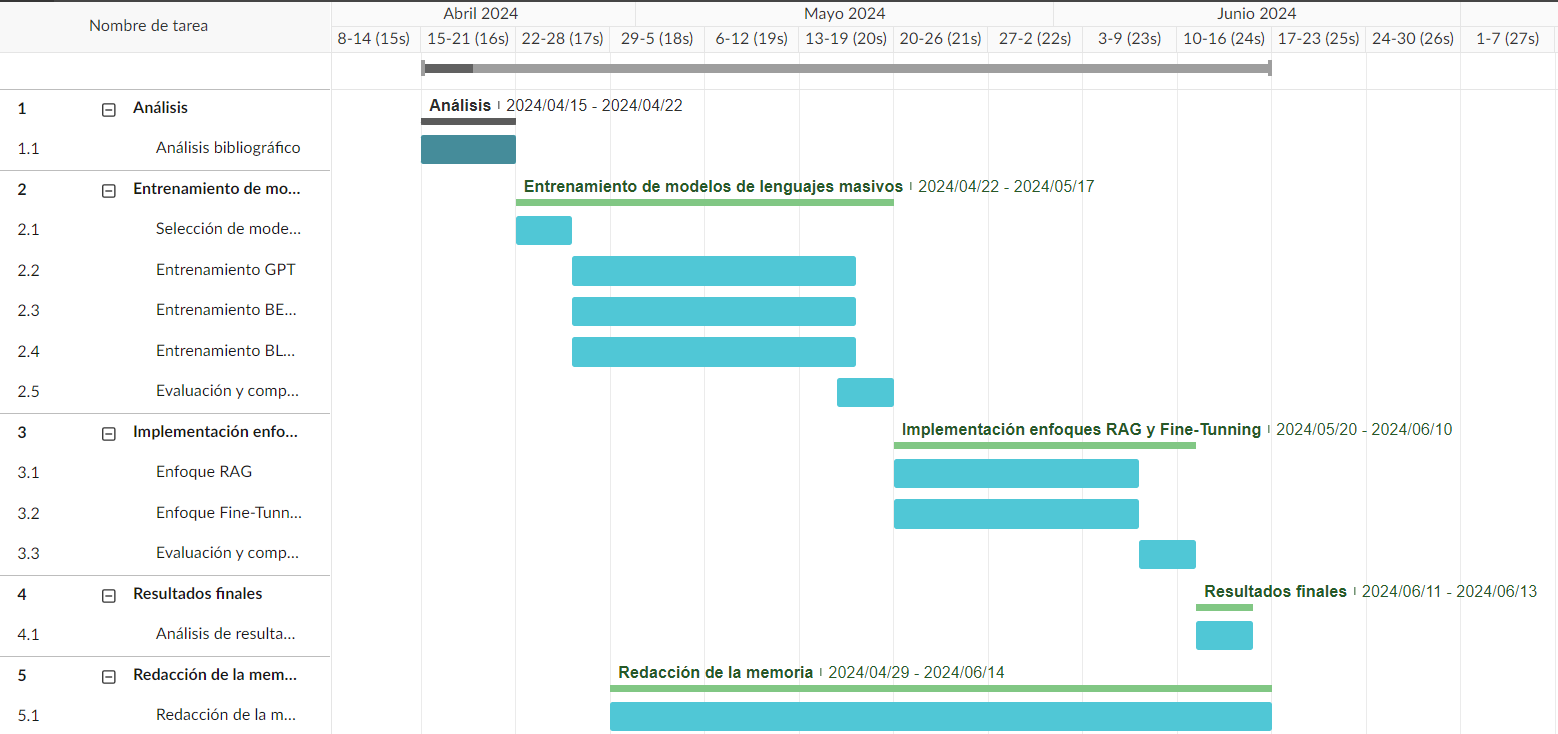
\includegraphics[width=\linewidth,height=\textheight,keepaspectratio]{imaxes/3_DiagramaGantt.png}
  \caption{Diagrama de Gantt del proyecto.}
  \label{fig:3_DiagramaGantt}
\end{figure}


\subsection{Fases}

La primera fase, \textbf{Análisis}, contiene 1 tarea:
\begin{itemize}
    \item \textbf{Tarea 1.1: Análisis bibliográfico.} En esta tarea se recopiló la información fundamental para iniciar el desarrollo del proyecto, incluyendo las tecnologías empleadas, la comprensión del dominio del problema, entre otros aspectos relevantes. Duración 1 semana y esfuerzo 40h.
\end{itemize}

La siguiente fase es \textbf{Entrenamiento de modelos de lenguajes masivos}, contiene 5 tareas:
\begin{itemize}
    \item \textbf{Tarea 2.1: Selección de modelos y conjunto de datos.} Implica elegir los modelos más apropiados y un conjunto de datos adecuado que nos facilite la realización de pruebas de manera óptima. Duración 3 días y esfuerzo 24h.
    \item \textbf{Tarea 2.2: Entrenamiento \acrshort{GPT}.} Entrenar el modelo \acrshort{GPT} utilizando el conjunto de datos seleccionado con el fin de obtener resultados satisfactorios y aprovechar al máximo la capacidad de este modelo de lenguaje masivo.
    Duración 2 semanas y esfuerzo 20h.
    \item \textbf{Tarea 2.3: Entrenamiento \acrshort{LLaMA}.} Entrenar el modelo \acrshort{LLaMA} utilizando el conjunto de datos seleccionado con el fin de obtener resultados satisfactorios y aprovechar al máximo la capacidad de este modelo de lenguaje masivo.
    Duración 2 semanas y esfuerzo 20h.
    \item \textbf{Tarea 2.4: Entrenamiento Mixtral.} Entrenar el modelo Mixtral utilizando el conjunto de datos seleccionado con el fin de obtener resultados satisfactorios y aprovechar al máximo la capacidad de este modelo de lenguaje masivo.
    Duración 2 semanas y esfuerzo 20h.
    \item \textbf{Tarea 2.5: Evaluación y comparativa de resultados.} Analizar y evaluar los resultados obtenidos por los diferentes modelos.
    Duración 3 días y esfuerzo 18h.
\end{itemize}

La siguiente fase, \textbf{Implementación de los enfoques \acrshort{RAG} y Fine-Tuning}, tiene 3 tareas:
\begin{itemize}
    \item \textbf{Tarea 3.1: Implementación enfoque \acrshort{RAG}.} Implementación del enfoque RAG en el proyecto, configurando y desarrollando el modelo de generación de código utilizando \acrfull{RAG} como base, con ajustes y personalizaciones para adaptarse a los requisitos del proyecto. Duración 1'5 semanas y esfuerzo 22'5h.
    \item \textbf{Tarea 3.2: Implementación enfoque Fine-Tuning.}
     Ajustar un modelo de lenguaje preentrenado para que se especialice en generar código, adaptándolo específicamente para las necesidades de este proyecto con el enfoque Fine-Tuning. Duración 1'5 semanas y esfuerzo 22'5h.
     \item \textbf{Tarea 3.3: Evaluación y comparativa de resultados.} Analizar los resultados obtenidos y las conclusiones relacionadas con la eficacia de cada enfoque utilizado en el proyecto. Duración 3 días y esfuerzo 15h.
\end{itemize}

La siguiente fase, \textbf{Resultados finales}, tuvo una sóla tarea:
\begin{itemize}
    \item \textbf{Tarea 4.1: Análisis de resultados finales.} Analizar los resultados obtenidos en todo el proyecto y obtener las conclusiones del proyecto. Duración 3 días y esfuerzo 15h.
\end{itemize}

Finalmente, tenemos la fase \textbf{Redacción de la memoria}, con una única tarea:
\begin{itemize}
    \item \textbf{Tarea 5.1: Redacción de la memoria.} Actividad llevada a cabo durante todo el proyecto para mantener actualizada la memoria con los avances realizados. Duración 3'5 semanas y esfuerzo 35h.
\end{itemize}

\section{Tablero Kanban}
Para obtener una visión más clara del progreso del proyecto, se ha optado por utilizar un \textbf{tablero Kanban} \cite{tableroKanban} para el seguimiento y la realización de las tareas. En la figura \ref{fig:3_TableroKanban}  se pueden observar todas las tareas por realizar y su estado actual. Una ventaja de utilizar este tablero es su integración con el Diagrama de Gantt, de modo que cualquier cambio en la estimación del tiempo de una tarea se reflejará automáticamente en el otro.

\begin{figure}[h]
  \centering 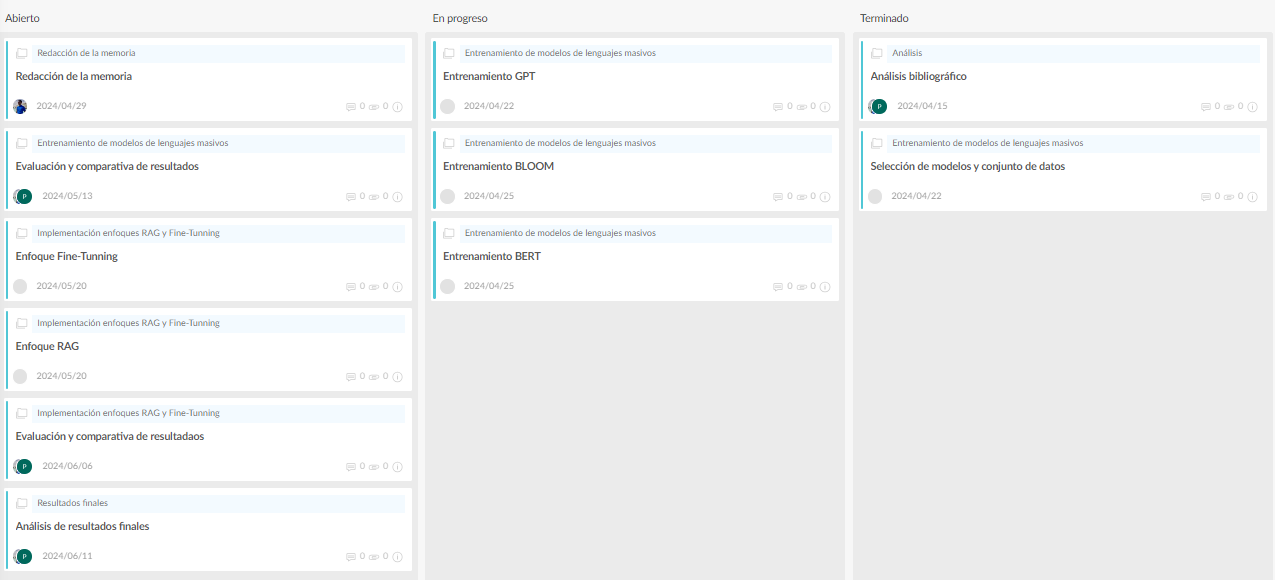
\includegraphics[width=\linewidth,height=\textheight,keepaspectratio]{imaxes/3_TableroKanban.png}
  \caption{Tablero Kanban del proyecto en desarrollo.}
  \label{fig:3_TableroKanban}
\end{figure}

\section{Estimación de costes}
Al calcular el coste del proyecto, se consideraron el tiempo dedicado, los recursos humanos necesarios y los materiales utilizados.

\subsection{Recursos humanos}
Al calcular el costo del proyecto, se parte del supuesto de que se lleva a cabo a tiempo completo, sin interrupciones, lo que equivale a una jornada de 40 horas semanales o 160 horas mensuales. Por lo tanto, considerando una duración total del proyecto de 360 horas y una semana laboral de 40 horas, se estima una duración de 9 semanas.

Para un desarrollador junior con un sueldo por hora de 11€, el costo total del trabajo sería de \textbf{3960€}.

Por otro lado, el tutor que desempeña la función de \acrfull{PO} tiene un sueldo de 30€ por hora. Dado que el proyecto se extiende a lo largo de 9 semanas y se realizan reuniones semanales de 1 hora, con una revisión final adicional de 10 horas, el costo total del \acrshort{PO} sería de \textbf{570€}.

\subsection{Recursos materiales}

La gran mayoría del software utilizado es software libre, por lo que no hemos tenido que pagar licencias para su uso. En el caso del software privativo, se han utilizado versiones gratuitas, excepto en el caso del \acrshort{API} de OpenAI \cite{APIOpenApi}, donde el costo depende del número de \gls{token}s utilizados y se estima en \textbf{20€}.

En cuanto al equipo informático, no se ha agregado ningún costo, ya que los equipos ya están completamente amortizados.

Por otro lado, en cuanto a los gastos de electricidad e internet, la electricidad representa un costo de \textbf{80€} por aproximadamente 3 meses de trabajo, mientras que el acceso a internet supone un costo de 23€ al mes, es decir, \textbf{69€} en total.


\subsection{Coste total}

En la siguiente tabla ~\ref{tab:Coste total proyecto}  se realiza un desglose del costo total del proyecto.

\begin{table}[hp!]
  \centering
  \rowcolors{2}{white}{udcgray!25}
  \begin{tabular}{c|c}
  \rowcolor{udcpink!25}
  \textbf{Concepto} & \textbf{Coste} \\\hline
  \textit{Desarrollador junior} & 3960€ \\
  \textit{\acrlong{PO}} & 570€ \\
  \textit{\acrshort{API} de OpenAI} & 20€ \\
  \textit{Electricidad} & 80€ \\
  \textit{Internet} & 69€ \\
  \textit{\textbf{COSTE TOTAL}} & \textbf{4699€} \\
  \end{tabular}
  \caption{Tabla con el desglose del coste total.}
  \label{tab:Coste total proyecto}
\end{table}